\documentclass[11pt]{report}
    \title{\textbf{Workshop Programming Languages: Nim}}
    \author{Niklas Peter}
    \date{}
    
    \addtolength{\topmargin}{-3cm}
    \addtolength{\textheight}{3cm}
\usepackage{graphicx}
\begin{document}

\maketitle
\tableofcontents


\chapter{Einleitung}
\section{Einleitung}
In diesem Bericht möchte ich die Programmiersprache Nim vorstellen. Ich werde zeigen, welche Merkmale und Eigenschaften sie hat und wie sie sich von anderen Programmiersprachen unterscheidet. Des Weiteren teile ich meine Erfahrungen mit der Verwendung von Nim in einem Programmierprojekt. Genauer gesagt die Verwendung zur Entwicklung eines simplen Klons des Kommandozeilen Werkzeugs \textbf{grep}, welches zur Suche bestimmter Zeichenketten in Dateien verwendet wird.



\chapter{Vorstellung der Sprache}

\section{Entstehung}
Andreas Rumpf hat 2005 mit der Entwicklung der Sprache, die effizient, ausdrucksvoll und elegant sein sollte, angefangen. In 2008 hat er sein Projekt, damals noch Nimrod genannt, veröffentlicht. Mit Veröffentlichung der Version 0.10.2 im Dezember 2014 wurde Nimrod zu Nim umbenannt.\footnote{https://nim-lang.org/blog/2014/12/29/version-0102-released.html} Am 23. September 2019 kam schließlich Version 1.0 raus. Ab diesem Zeitpunkt garantiert Nim eine gewisse Stabilität, indem zwischen Hauptversionen keine größeren Änderungen eingeführt werden, die im schlimmsten Fall Bugs und weiterem Fehlverhalten führen könnte.\footnote{https://nim-lang.org/blog/2019/09/23/version-100-released.html} Mittlerweile wird Nim von einem Team bestehend aus Andreas Rumpf und weiteren Freiwilligen weiter entwickelt. Die Programmiersprache ist quelloffen und wird unter der MIT Lizenz veröffentlicht.

\subsection{Einflüsse anderer Sprachen}
Nims Speichermanagement ist inspiriert von C++ und Rust. Es ist deterministisch und anpassbar durch Destruktoren und Move Semantics.\footnote{https://nim-lang.org/}
\newline
Nim kombiniert Python's leserliche Syntax, Ada's starkes statisches Typisierungssystem und Lisp's flexibles Macrosystem.\footnote{https://www.youtube.com/watch?v=-9SGIB946lw}

\subsection{Syntax}
Die Syntax von Nim gleicht der von Python. Das bedeutet, Codeblöcke werden durch Einrückung ausgedrückt. Viele  Schlüsselwörter sind identisch zu denen von Python. So wird beispielsweise im Gegensatz zu anderen Programmiersprachen bei einer Verneinung einer Bedingung kein Ausrufezeichen sondern das Schlüsselwort \emph{not} verwendet. Anders als Python setzt Nim auf statische Typisierung, allerdings wird einfache Typ Umwandlungen gesetzt.
\newline
Um verschiedene Programmierstile (zum Beispiel camelCase oder snake\verb|_|case) zu ermöglichen, ist Nim \emph{style-insensitive}. Das bedeutet, zwei Bezeichner (zum Beispiel Variablennamen) mit unterschiedlicher Groß- und Kleinschreibung und mit oder ohne Unterstrich können als der selbe Bezeichner interpretiert werden, so lange der erste Buchstabe identisch ist. Dies Ermöglicht eine Mischung an Stilen über Bibliotheken ohne Probleme.

Zusätzlich unterstützt Nim Uniform Function Call Syntax (UFCS). Dabei können Funktionen wie Methoden aus objektorientierten Sprachen benutzt werden. Hierzu wird der Empfänger als erster Parameter und die gegebenen Argumente als die restlichen Parameter verwendet. Beispiel:
\newline
\emph{x = multiply(y, z)} entspricht \emph{x = y.multiply(z)}.
\newline
Das ist besonders nützlich, wenn mehrere Funktionen aneinander kettet werden:
\newline
\emph{x = x.muliply(y).multiply(z)}

\subsection{Allgemeines}
Nim ist wie Python eine imperative Sprache. Allerdings ist sie nicht wie Python auch eine Interpreter Sprache, sondern kompiliert zu C. Das bringt Vorteile bei der Performance Gegenüber Python bei ungefähr gleichbleibender Einfachheit der Programmierung aufgrund der Syntax.

Ähnlich wie bei Rust, kann man sich bei der Definition einer Variable entscheiden, ob sie \emph{immutable} sein soll, indem man statt dem Schlüsselwort \emph{var} das Schlüsselwort \emph{let} benutzt. Dadurch kann der Variable nur einmal ein Wert zugewiesen werden. Das ist dann wichtig, wenn man ungewollte Speicherzugriffe vermeiden möchte.

\section{Nutzung heute}
Aufgrund der einfachen Syntax eignet sich Nim hervorragend zum Shell Scripting.
Aber auch für anspruchsvollere Projekte wie Frontend und Backend Entwicklung für Webdienste, Machine Learning oder sogar eingebettete Systeme ist Nim geeignet, da Nim zu C, C++ und JavaScript kompilieren kann.

Aufgrund der vielen Einsatzmöglichkeiten gibt es jede Menge Projekte, die in Nim geschrieben wurden. Im Folgenden eine kleine Auswahl an Projekten:
\begin{description}
\addtolength{\itemindent}{0.60cm}
\item[Chroma] Eine Bibliothek um mit Farben und Farbräumen zu arbeiten. Einfache Transformierung von Farben.\footnote{https://github.com/treeform/chroma}
\item[dimscord] Ein Discord Bot\footnote{https://github.com/krisppurg/dimscord}
\item[godot-nim] Nim Bindings für die Game Engine Godot\footnote{https://github.com/pragmagic/godot-nim}
\item[httpx] Ein plattformübergreifender Web Server\footnote{https://github.com/ringabout/httpx}
\item[netty] Eine UDP Verbindungsbibliothek für Spiele in Nim\footnote{https://github.com/treeform/netty}
\item[nim-regex] Eine Bibliothek, um reguläre Expressionen zu parsen, kompilieren und auszuführen. Zur Laufzeit und zur Kompilierungszeit.\footnote{https://github.com/nitely/nim-regex}
\item[nitter] Ein Front End für Twitter.\footnote{https://github.com/zedeus/nitter} Vermutlich eines der am weit verbreitetsten Projekte, welches in Nim geschrieben wurde.
\item[rod] Eine plattformübergreifende 2D und 3D Game Engine\footnote{https://github.com/yglukhov/rod}
\item[Stardust] Ein Online Spiel im Browser\footnote{https://stardust.dev/play/}
\end{description}


\section{Programmierungsparadigmen}
\subsection{Funktionale Programmierung}
Nim unterstützt funktionale Programmierung und es gibt First-Class-Funktionen. Diese können anderen Funktionen als Argument übergeben werden, von einer anderen Funktion als Wert zurückgegeben werden, einer Variables zugewiesen werden, in einer Datenstruktur gespeichert werden und zur Laufzeit erzeugt werden.\footnote{https://de.wikipedia.org/wiki/First-Class-Funktion}
\newline
Zur Kompilierzeit hat man die Möglichkeit Funktionen auf Side Effects zu überprüfen. Dazu markiert man Funktionen mit dem Schlüsselwort \emph{func} oder man beschriftet eine Prozedur mit \verb|{.noSideEffect.}|. Wenn solche Side Effects gefunden werden, scheitert die Kompilierung. Zu diesen Side Effects gehören Mutation, globaler Zugriff oder Modifikation, asynchroner Code, Threaded Code und Input/Output. In zukünftigen Versionen ist es geplant, Mutationen durch \emph{ref} und \emph{ptr} ebenfalls zu verbieten.\footnote{https://forum.nim-lang.org/t/9716}
\newline
Es ist möglich, verschiedene Funktionen aneinander zu ketten. Dabei wird das Ergebnis der ersten Funktion an die nächste Funktion als Parameter weitergegeben. In Abbildung 2.1 ist eine solche Verkettung zu sehen.
\begin{figure}[htp]
\centering
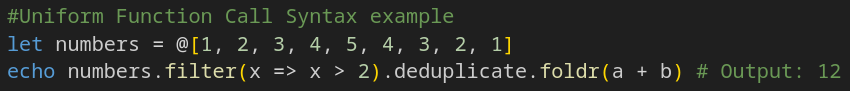
\includegraphics[scale=0.40]{images/image4.png}
\caption{UFCS Beispiel}
\label{}
\end{figure}
\newline
Außerdem unterstützt Nim Pattern Matching, welches durch Marcos umgesetzt wird. Darunter versteht man Verfarhen, die durch vorgegebene Muster diskrete Strukturen oder Teilmengen einer diskreten Struktur identifizieren.\footnote{https://en.wikipedia.org/wiki/Pattern\_matching}

\subsection{Objektorientierte Programmierung}
In erster Linie ist Nim eine imperative und funktionale Sprache. Trotzdem kann darüber hinaus auch objektorientiert programmierst werden. Allerdings mit eingeschränktem Umfang.
Ein Objekt wird mit dem Schlüsselwort \emph{type} initialisiert und ähneln \emph{structs} aus der Programmiersprache C.
\begin{figure}[htp]
\centering
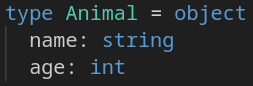
\includegraphics[scale=0.50]{images/image1.png}
\caption{Objekt Deklaration}
\label{}
\end{figure}
In Abbildung 2.2 wird die Deklaration des Objekts \emph{Animal} mit den Feldern \emph{name} und \emph{age} gezeigt. Beim Erzeugen eines Objektes können gleich die Werte für die Felder mit angegeben werden. Werden diese Werte nicht mit angegeben, werden sie automatisch auf 0 oder, im Falle eines Strings, auf einen leeren String gesetzt. Das ist wichtig, da es im Gegensatz zu anderen objektorientierten Sprachen keine Kontruktor- oder Dekonstruktor-Methoden gibt und so mit den Werten in Funktionen, die einen Parameter verlangen, gerechnet werden kann. Selbst wenn die Werte auf 0 gesetzt wurden, können sie trotzdem nachträglich noch verändert werden. Es sei denn, man initialisiert ein Objekt mit dem Schlüsselwort \emph{let}, welches die Werte der Felder unveränderbar machen.

Es ist möglich ein Objekt zu referenzieren. Anstatt das Objekt auf dem \emph{Stack} zu speichern, wird bei einer Referenz nur auf eine Stelle des \emph{Heaps} im Speicher gezeigt. Dafür wird das Schlüsselwort \emph{ref} verwendet.\footnote{https://nim-by-example.github.io/types/objects/}
Referenzen sind für die Vererbung erforderlich. Um Vererbung überhaupt möglich zu machen, muss das Objekt von \emph{RootObj} erben. In dem Beispiel mit dem \emph{Animal} Objekt würde das so aussehen: \emph{type Animal = object of RootObj}. Um von diesem Objekt zu erben, deklariert man ein weiteres Objekt wie folgt: \emph{type Pet = ref object of Animal}.
Es ist möglich während der Laufzeit den Typ eines Objektes zu überprüfen.
Dies geschieht mit dem \emph{of} Operator, welcher vergleichbar mit dem Operator \emph{instanceof} in Java ist.\footnote{https://nim-lang.org/docs/manual.html}

Methoden der Objekte werden nicht im Kontext des Objektes definiert, sondern können einfach als Prozedur mit \emph{proc} implementiert werden. Durch UFCS können die Methoden dann, wie von anderen objektorientierten Sprachen gewohnt, verwendet werden: \emph{instance.method()} anstatt \emph{method(instance)}.
Um die Werte eines Objekts beispielsweise mithilfe von Setter-Methoden zu verändern, muss das Argument für das Objekt der Methode durch \emph{var} gekennzeichnet werden, da die Argumente von Prozeduren standardmäßig unveränderbar sind und \emph{var} diese Beschränkung aufhebt.
In Verbindung mit Vererbung können statt Prozeduren \emph{proc} auch Methoden \emph{method} benutzt werden. Der Vorteil liegt darin, dass Methoden überschrieben werden können. Dazu benutzt man den Typ des Subtyps in den Parametern. Man sollte allerdings nur begrenzt darauf zurückgreifen, da Methoden eine dynamische Bindung und Prozeduren eine statische Bindung haben und diese performanter ist gegenüber der dynamischen ist.\footnote{https://nim-by-example.github.io/oop/}


\subsection{Metaprogrammierung}
Metaprogrammierung ist die Verwendung von Computerprogrammen, die beim Prozess der Programmierung mitarbeiten und so Fehler vermindern und die Effektivität steigern.\footnote{https://de.wikipedia.org/wiki/Metaprogrammierung} In Nim stehen dazu Generics, Templates und Macros zur Verfügung.

Generics erlauben die Parametrisierung von Prozeduren, Iteratoren und Typen mit Typ Parametern, wodurch die Typisierung erst später stattfindet. Dadurch wird sich duplizierender Code verringert, Parameter werden in eckigen Klammern geschrieben und sie erweisen sich gerade für effiziente typsichere Container als sehr nützlich.\footnote{https://nim-lang.org/docs/tut2.html}

Ein Template wird wie eine Prozedur aufgerufen. Sie sind eine einfache Form von Makros und eine Mechanik, um Teile vom Code im semantischen Durchgang im Kompilierer auszutauschen und zu verarbeiten. Beispielsweise sind Nim's \emph{!=}, \verb|>|, \verb|>=|, \emph{in}, \emph{notin} und \emph{isnot} Operatoren als Templates umgesetzt worden.\footnote{https://nim-lang.org/docs/manual.html}
\begin{figure}[htp]
\centering
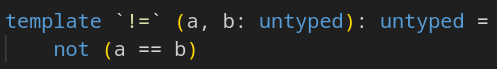
\includegraphics[scale=0.50]{images/image2.png}
\caption{Umsetzung des != Operators in Nim's System Modul}
\label{}
\end{figure}

Ein Macro ist eine Funktion, die bei der Kompilierung ausgeführt wird und einen Nim Syntax Tree in einen anderen transformiert.\footnote{https://nim-lang.org/docs/tut3.html} Macros eignen sich gut, um den Code übersichtlicher zu gestalten.

\subsection{Foreign function interface}
Ein mächter Teil von Nim ist das FFI (Foreign function interface). Diese Schnittstelle erlaubt es dem Programmierer, innerhalb seines Nim Programmes auf in anderen Programmiersprachen geschriebenen Bibliotheken zuzugreifen, indem diese importiert und deren Funktionen dann ganz normal verwendet werden können. Nim unterstützt Bibliotheken in den Sprachen C, C++, Objective-C und JavaScript. Allerdings können nicht alle vier Sprachen gleichzeitig mit eingebunden werden. Man muss sich zwischen C/C++/Obj-C oder JavaScript entscheiden, denn JavaScript ist inkompatibel zu den anderen drei Sprachen. Diese drei Sprachen können aber gleichzeitig in Nim verwendet werden, da C++ und Obj-C die ABI von C unterstützen.
Nim unterstützt sowohl statisches Linken, bei dem die importierte Bibliothek in das Programm eingebettet wird, als auch dynamisches Linken, bei dem die Bibliothek auf dem PC des Nutzers installiert sein muss. Nim bevorzugt dynamisch gelinkte Bibliotheken.
\begin{figure}[htp]
\centering
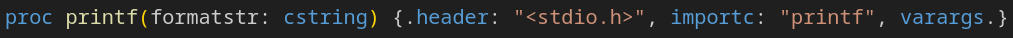
\includegraphics[scale=0.40]{images/image3.png}
\caption{Die Funktion printf aus der C Bibliothek stdio}
\label{}
\end{figure}
Wie in Abbildung 2.4 zu sehen, wird gegebenenfalls eine Typkonvertierung benötigt, beispielsweise bei \emph{cstring}, denn Nims Typen sind teilweise nicht mit denen von C kompatibel.\footnote{https://livebook.manning.com/book/nim-in-action/chapter-8/102}

\subsection{Parallelisierung und Nebenläufigkeit}
Um Parallelisierung durch Threads zu aktivieren, muss das Programm mit der Option \emph{--threads:on} kompiliert werden. Eine Funktion, die in einem Thread ausgeführt wird, sollte mit dem Pragma \verb|{.thread.}| gekennzeichnet werden. Eine Thread Prozedur kann durch \emph{spawn()} oder \emph{createThread()} gestartet werden und auf laufende Threads kann mit \emph{joinThreads()} gewartet werden.
Anstatt Threads einzeln zu starten, kann die \emph{threadpool} Bibliothek verwendet werden. Dort stehen strukturierter Parallelismus mit dem Statement \emph{parallel} und unstrukturierter Parallelismus mit dem Statement \emph{spawn} zur Verfügung. Die Verwendung dieser Statements wird durch gewisse Regeln eingeschränkt, um gewisse Sicherheiten zu gewährleisten. Beispielsweise sind Speicherzugriffe eingeschränkt und jeder Thread hat seinen eigenen Garbage Collector.

Nebenläufigkeit wird durch async/await Syntax erzielt. Eine Prozedur mit Nebenläufigkeit wird mit \verb|{.async.}| gekennzeichnet. Dadurch kann sie das \emph{await} Schlüsselwort verwenden, um auf asynchrone Prozeduren zu warten.


\section{Infrastruktur}
\subsection{Kompilierer}
Nims Kompilierer ist eine der großen Stärken der Sprache, da dieser standardmäßig zu schnellem und optimiertem C Code kompiliert. Das macht es einfach in Nim zu programmieren, da Python's Syntax, auf der Nim basiert, anfängerfreundlicher und effizienter ist als direkt in C zu programmieren.
Außerdem ist ein zu C kompiliertes Programm auch wesentlich schneller als ein interpretiertes Programm, wie es zum Beispiel bei Python der Fall ist.
Die Kompilierung zu Objektcode wird an einen externen Kompilierer abgegeben, um von bereits vorhandenen Optimierungen zu profitieren. Zu den unterstützten C Kompilierern zählen beispielsweise \emph{GCC (GNU Compiler Collection}), \emph{MinGW} und \emph{Clang}. Nim kann nicht nur Bibliotheken geschrieben in C, C++, Objective-C und JavaScript einbinden, sondern diese auch beim Kompilieren ausgeben. Das erleichtert die Verwendung von APIs (Application Programming Interface) in diesen Sprachen.
Ursprünglich war der Kompilierer in Pascal geschrieben. Doch 2008 wurde eine in Nim geschriebene Version des Kompilierers veröffentlicht, sodass dieser selbsttragend ist. Nim läuft auf Linux, Windows und MacOS aber auch der Export nach diesen Betriebssystemen wird von dem Kompilierer unterstützt, was gerade für Anwendungen im Bereich eingebetteter Systeme und mit unüblichen Architekturen von Nutzen ist.
Durch Cross-Compilation ist es möglich für Android, iOS oder sogar für die Nintendo Switch zu kompilieren.\footnote{https://nim-lang.org/docs/nimc.html}

Standardmäßig erstellt der Kompilierer ein Debug Build. Das ist für den Programmierer sehr nützlich, da dieses mehr Runtime Checks beinhaltet. Allerdings ist dieser Debug Build nicht für Schnelligkeit optimiert. Um schnellere Builds mit weniger Runtime Checks zu erstellen, wird die Option \emph{-d:release} benutzt. Mit der Option \emph{-d:danger} werden für maximale Schnelligkeit sämtliche Runtime Checks entfernt.

Der Kompilierer implementiert verschiedene Garbage Collectors. Eine Garbage Collection ist eine automatische Speicherverwaltung, die zur Vermeidung von Speicherproblemen beiträgt, indem zur Laufzeit versucht wird, nicht länger benötigte Bereiche im Speicher zu finden, um diese dann wieder freizugeben.
Einen Garbage Collector auszuwählen geht mit der Option \emph{--gc}. Wobei standardmäßig ORC verwendet wird. Dieser versucht durch das automatische Zählen von Referenzen mit \emph{move} Semantik Optimierungen freizugebenden Speicher zu identifizieren und bietet voll-deterministische Performance für harte Echtzeitsysteme. Referenzzyklen, die zu Memory Leaks führen würden, werden durch einen Zyklus Collector vermieden.
Es ist möglich auf einen Garbage Collector zu verzichten, indem man die Option \emph{--gc:none} angibt. Hierbei gibt es keine Speichermanagement Strategie und es wird kein Speicher mehr automatisch freigegeben. Der Entwickler muss sich also in diesem Fall selbst um die Speichernutzung in seinem Programm kümmern.


\subsection{Entwicklungswerkzeuge}
Die folgenden Werkzeuge werden mit der Standard Nim Installation automatisch mitgeliefert.\footnote{https://nim-lang.org/docs/tools.html}

\subsubsection{Nimble}
Das wohl wichtigste Entwicklungswerkzeug für Nim ist Nimble. Es ist Nims Paketmanager. Entwickelt wurde Nimble von einem der Hauptentwickler Nims Dominik Picheta und ist seit 2015 Nims offizieller Paketmanager. Nimble Pakete werden durch .nimble Dateien definiert, welche Informationen über die Paketversion, Autoren, Lizenzen, Abhängigkeiten und mehr enthalten.
.nimble Dateien unterstützen NimScript, einen Teil von Nims Syntax. Mit diesen Skripten können Test Prozeduren verändert werden und benutzerdefinierte Aufgaben geschrieben werden.
Eine Liste mit verfügbaren Paketen im JSON (\emph{JavaScript Object Notation}) Format wird im nim-lang/packages Repository auf Github frei zur Verfügung gestellt.\footnote{https://github.com/nim-lang/packages/blob/master/packages.json} Diese Liste beinhaltet die Namen und Repositories der verschiedenen Pakete. Da es kein zentrales Repository mit allen Paketen gibt sondern jeder sein eigenes Repository hosten kann, ist eine gute Zugänglichkeit des Ökosystems gegeben.
Nimble benötigt Git um richtig zu funktionieren. Mit dem Commandline Interface lassen sich Pakete der Module installieren, aktualisieren und deinstallieren.

\subsubsection{atlas}
\emph{atlas} ist ein einfaches Paket Kloner Werkzeug. Es verwaltet eine isolierte Arbeitsumgebung und beinhaltet Projekte und Abhängigkeiten. Es ist mit Nimble kompatibel, da es das Nimble Datei Format unterstützt.
Es gibt drei Konzepte: Arbeitsflächen, Projekte und Abhängigkeiten.

Jede Arbeitsfläche ist isoliert und zwischen den Arbeitsflächen wird nichts geteilt. Jede Arbeitsfläche ist ein Verzeichnis und beinhaltet eine \emph{atlas.workspace} Datei. Mit \emph{atlas init} lassen sich Arbeitsflächen in dem derzeitigen Arbeitsverzeichnis erstellen.

Eine Arbeitsfläche enthält ein oder mehrere Projekte. Diese Projekte können sich gegenseitig benutzen und es ist einfach mehrere Projekte gleichzeitig zu entwickeln.

Auf einer Arbeitsfläche kann es ein \verb|_deps| Verzeichnis geben, in dem die Abhängigkeiten aufbewahrt werden. Der einzige Unterschied zwischen einem Projekt und einer Abhängigkeit ist der Aufbewahrungsort. Für eine Abhängigkeitsresolution hat ein Projekt stets die höhere Priorität.

Atlas kümmert sich für den Entwickler nur um die zwei Dateien \emph{project.nimble} und \emph{nim.cfg}. Ansonsten wird alles so gelassen wie es ist.\footnote{https://nim-lang.org/docs/atlas.html}

\subsubsection{Hot code reloading}
Durch die hotCodeReloading Option wird ein spezieller Kompilierungsmodus aktiviert, wodurch Änderungen im Code automatisch auf ein laufendes Programm angewendet werden können. Das Neuladen des Codes passiert mit individuellen Modulen. Wenn ein Modul neu geladen wird, werden jegliche neu hinzugefügte globale Variablen initialisiert aber der restliche top-level Code in diesem Modul wird nicht erneut ausgeführt und der aktuelle Zustand von allen bereits existierenden globalen Variablen bleibt erhalten. Zurzeit funktioniert Hot Code Reloading nicht für das Hauptmodul selbst, weswegen ein Helfer Modul benutzt werden muss. Es gibt spezielle Event Handhaber, die vor und nach dem Reload ausgeführt werden, um den Zustand einer bestimmten Variable zu ändern oder um die Ausführung bestimmter Statements zu erzwingen. Diese Handhaber werden mit \emph{beforeCodeReload} und \emph{afterCodeReload} aufgerufen. Um Hot Code Reloading zu verwenden muss das hotcodereloading Modul importiert werden und beim Kompilieren die Option \emph{--hotcodereloading:on} gesetzt sein.\footnote{https://nim-lang.org/docs/hcr.html}

\subsubsection{Document generator}
Der in den Nim Kompilierer eingebaute Dokument Generator \emph{nim doc} generiert HTML (\emph{Hyptertext Markup Language}), Latex und JSON Dokumentation von \emph{.nim} Quelldateien und Projekten. Der Output beinhaltet die Modulabhängigkeiten (Imports), alle obersten Dokumentationskommentare (\verb|##|) und exportierte Symbole (*) inklusive Prozeduren, Typen und Variablen.
Man kann eine Dokumentation in HTML mit \emph{nim doc} \verb|<|\emph{filename}\verb|>|\emph{.nim} generieren.\footnote{https://nim-lang.org/docs/docgen.html}

\subsubsection{Nimsuggest IDE support}
Da Nim sehr schnell ist, bietet es sich an, den Texteditoren externe Abfragen über den geschrieben Quellcode zur Verfügung zu stellen.
Durch das \emph{nimsuggest} Werkzeug kann jede Entwicklungsumgebung \emph{.nim} Quelldateien abfragen und nützliche Informationen wie Definitionen von Symbolen oder Vorschläge zur automatischen Vervollständigung erhalten.\footnote{https://nim-lang.org/docs/nimsuggest.html} Unterstützung werden Editoren wie beispielsweise VSCode, Emacs, Vim und viele weitere.\footnote{https://github.com/nim-lang/Nim/wiki/Editor-Support}

\subsubsection{C2nim}
C2nim ist ein ANSI C/C++ zu Nim Quellcode Übersetzer. Das Werkzeug übersetzt C Header Files nach Nim. Der Output ist leserlicher Nim code, welcher noch durch den Entwickler überarbeitet werden sollte. C2nim ist dafür gedacht C Code Fragmente zu übersetzen und folgt daher keinen inculde Dateien. Nicht jeder C/C++ Code kann übersetzt werden, da Konstrukte in C/C++ existieren, die in Nim nicht dargestellt werden können. Mit der Option --nep1 generiert C2nim Nim Code, der den offiziellen Style Guides folgt.\footnote{https://github.com/nim-lang/c2nim/blob/master/doc/c2nim.rst}

\subsubsection{niminst}
Ein Werkzeug zum Generieren eines Installers für ein Nim Programm. Zurzeit können nur ein altmodischer grafischer Installer für Windows sowie Installations- und Deinstallationsskripte für Linux/Unix erstellt werden. Unterstützung für Paketmanager unter Linux ist ebenfalls geplant.
Zur Erstellung des Installers liest niminst eine Konfigurationsdatei aus, die alle notwendigen Informationen für den Installer für die jeweiligen Betriebssysteme enthält.\footnote{https://nim-lang.org/docs/niminst.html}

\subsubsection{nimgrep}
Ein Nim Such- und Ersetzungswerkzeug in der Kommandozeile. Es kann nach Regex und Peg Patterns suchen und kann ganze Verzeichnisse auf einmal durchsuchen. Nimgrep hat eine besonders gute Unterstützung für Nim's Style Insensibilität durch die \emph{-y} Option.

\subsubsection{nimpretty}
Mit \emph{nimpretty} lassen sich Nim Quelldateien verschönern, indem Code nach den offiziellen Style Guides formatiert wird.\footnote{https://nim-lang.org/docs/tools.html}

\subsubsection{testament}
testament ist ein fortgeschrittener Unittest Runner für Nim Tests, welcher für die Entwicklung Nim's selbst verwendet wird. Es bietet Prozess Isolation für Tests, kann Statistiken über Testfälle und HTML Berichte generieren. Außerdem werden mehrere Programmiersprachen unterstützt.\footnote{https://nim-lang.org/docs/testament.html}

\subsubsection{koch}
Das koch Programm ist ein Wartungsskript. Es ist als Ersatz für \emph{make} und Shell Scripting gedacht mit dem Vorteil, dass es viel portabler ist. Es ist hauptsächlich zum Bauen des Kompilierers gedacht aber es kann auch anderweitig benutzt werden.
\newline\newline\newline
Andere nützliche Werkzeuge, die nicht automatisch mitgeliefert werden:

\subsubsection{choosenim}
Choosenim ist ein Werkzeug, das die Installation und Benutzung mehrerer Versionen des Nim Kompilierers ermöglicht. Man kann jede \emph{stable} oder \emph{development} Version mit der Kommandozeile installieren und schnell und einfach zwischen ihnen wechseln.

\subsubsection{nimpy}
Nimpy ist eine Bibliothek, die Python in Nim integriert.\footnote{https://github.com/yglukhov/nimpy}

\subsubsection{Pixie}
Pixie ist eine umfangreiche 2D Grafik Bibliothek für Nim.\footnote{https://github.com/treeform/pixie}

\subsubsection{nimterop}
Nimterop ist ein Paket mit dem Ziel die Interoperabilität makellos zu gestalten. Es automatisiert die Erstellung von C Wrappern für Nim's FFI.
C++ Unterstützung ist ebenfalls geplant.\footnote{https://github.com/nimterop/nimterop}

\subsection{Bibliotheken}
Bei Nim Bibliotheken wird zwischen Pure und Impure unterschieden.
Pure bedeutet, dass die Module der Bibliothek ausschließlich in Nim geschrieben wurden ohne die Verwendung von Wrappern, um auf Bibliotheken zuzugreifen, die in anderen Sprachen geschrieben wurden.
Bei Impure sind die Nim Module auf Code aus Bibliotheken angewiesen, die in anderen Programmiersprachen geschrieben wurden wie zum Beispiel C oder C++.

Die Standardbibliothek wurde ausschließlich in Nim geschrieben und beinhaltet Module für grundlegende Aufgaben, wie zum Beispiel für den Umgang mit Dateien, die Interaktion mit dem Betriebssystem oder wichtige Formeln aus der Mathematik.

Auf \emph{https://nimble.directory} werden viele externe Bibliotheken mit kurzer Beschreibung vorgestellt.\footnote{https://nimble.directory/}

Nim kann Bibliotheken in den Sprachen C, C++, Objective-C und JavaScript nativ in das Programm einbinden. Aber auch auf Bibliotheken in anderen Sprachen kann mithilfe von Language Bindings zugegriffen werden. Für Bibliotheken wie GTK, OpenSSL und Vulkan gibt es bereits solche Bindings.


\subsection{Dokumentation}
Obwohl Nim nicht die weit verbreitetste Sprache ist, verfügt sie über eine ausgesprochen gute und umfangreiche Dokumentation.
Es gibt mehrere Tutorials für Anfänger und Experten. Es wurden Tutorials extra für Programmierer, die schon C, Python oder JavaScript Erfahrung haben, erstellt. Dokumentation für die Standardbibliothek, inklusive der einzelnen Module, ist ebenfalls verfügbar.
Genauso wie Dokumentation für die einzelnen Bestandteile der Sprache, wie zum Beispiel die Bedienung des Kompilierers, der Aufbau der Syntax oder einfach nur wie man Nim installiert.
Außerdem werden auch die verschiedenen Entwicklungswerkzeuge, die vorgestellt wurden, im Detail erklärt.
Da Nim eine aktive Community hat, können andere Leute um Rat gefragt werden, sollten Probleme auftreten.



\chapter{Implementierung}
\section{Herangehensweise}
Das Programm wurde schrittweise in der Reihenfolge geschrieben, wie es später ausgeführt wird. Angefangen mit dem Einlesen der Parameter aus der Kommandozeile. Dafür werden die einzelnen Parameter zuerst in einer Sequenz gespeichert. Anschließend wird mit Hilfe einer for-Schleife Parameter für Parameter überprüft, ob es sich um eine valide Option des Programms handelt. Um das umzusetzen, habe wird ein Switch Statement verwendet. Wenn eine valide Option gefunden wurde, wird die entsprechende Variable im Programm auf True oder False oder auf den entsprechenden Wert gesetzt. Da es sich nicht bei allen Parametern gleichzeitig auch um Optionen handelt, wird unter den Parametern zwischen Optionen und Pattern oder Pfad unterschieden. Die Unterscheidung kann man einfach umsetzen, weil Optionen mit einem Bindestrich beginnen. Außerdem gibt das Programm dem Nutzer die Syntax vor, die verlangt, dass erst die Optionen angegeben werden, dann das Pattern und danach optional noch den Pfad beziehungsweise die Pfade, falls mehrere Orte durchsucht werden sollen.
Das heißt, das Programm kann davon ausgehen, dass der erste Parameter nach den Optionen das Pattern ist und alles, was dann noch folgt, als Pfad interpretiert wird. Die angegebenen Pfade werden in absolute Pfade umgewandelt, damit der Nutzer neben Dateien und Verzeichnissen im aktuellen Arbeitsverzeichnis auch beliebig andere Dateien von außerhalb angeben kann. Wenn kein Pfad angegeben wird, werden alle Dateien und Verzeichnisse im aktuellen Arbeitsverzeichnis durchsucht.

Damit die Suche nach dem Einlesen starten kann, wurde die Prozedur checkFiles geschrieben, welche eine Sequenz an Pfaden übergeben bekommt. In dieser Prozedur werden zuallererst die einzelnen Pfade in \emph{Pfad zu einer Datei} und \emph{Pfad zu einem Verzeichnis} unterteilt. Das wurde gemacht, damit zuerst die einzelnen Dateien untersucht und anschließen die Verzeichnisse rekursiv weiter nach weiteren Dateien und Verzeichnissen untersuchen werden können, indem die Prozedur checkFiles erneut mit den neuen Pfaden aufgerufen wird.

Um die einzelnen Dateien zu untersuchen, gibt es die checkFile Prozedur, welche zum Einen den Pfad zur Datei und zum Anderen das Pattern übergeben bekommt.
Bevor in der Datei nach dem Pattern gesucht werden kann, muss allerdings erst einmal überprüft werden, ob die Datei überhaupt Text enthält. Dafür wird im Programm der file-Befehl\footnote{https://darwinsys.com/file/} aufgerufen und anhand des MIME-Typs aus dessen Output wird gelesen, ob es sich bei der Datei um eine Textdatei handelt oder nicht. Wenn es keine Textdatei ist, wird sie übersprungen und nicht durchsucht.
\newline
Um eine Datei zu durchsuchen, wird Zeile für Zeile überprüft, ob diese das Pattern beinhaltet. Wenn das Pattern gefunden wurde, wird der Index der entsprechenden Zeile in einer Sequenz gespeichert. Außerdem wird bei jeder Datei gezählt, wie viele Zeilen sie hat, weil in einem späteren Schritt die letzte Zeile beziehungsweise das Ende wichtig wird.

Sobald alle Zeilen überprüft wurden und mindestens ein Treffer gefunden wurde, wird die nächste Prozedur aufgerufen: printResult. Ihr werden Pfad zur Datei, Anzahl aller Zeilen der Datei und die Sequenz der Indizes der Zeilen, in der das Pattern gefunden wurde, übergeben. Falls der Nutzer angegeben hat, dass das Ergebnis mit Kontext Zeilen ausgegeben werden soll, wird im nächsten Schritt die Sequenz mit den Indizes um jeweils den entsprechenden Kontext erweitert.
\newline
Wenn beispielsweise der Index 70 in der Sequenz beinhaltet ist und Kontext davor von 2 und Kontext danach von 3 erwünscht ist, werden die entsprechenden Indizes der Sequenz hinzugefügt, sodass nachher 68, 69, 70, 71, 72, 73 gemeinsam in der Sequenz sind.
\newline
Jetzt wird die Datei erneut Zeile für Zeile durchgegangen. Allerdings nicht, um sie nochmal nach dem Pattern zu durchsuchen, sondern wird hier bei jeder Zeile geschaut, ob ihr Index in der Sequenz mit beinhaltet ist. Wenn das der Fall ist, wird die Zeile ausgegeben. Hier kann ebenfalls unterschieden werden, ob es sich um eine Zeile mit Pattern handelt oder ob es nur eine Kontext Zeile ist, indem zusätzlich überprüft wird, ob der Index auch in der Sequenz bestehend nur aus den Zeilen mit Pattern und ohne Kontext Zeilen ist.
Gleichzeitig wird der Output entsprechend der Optionen gestaltet, je nachdem er farbig sein soll und mit oder ohne Heading.

Zusätzlich wurden noch ein paar Helferprozeduren geschrieben.
\newline
printHelp gibt den Syntax und alle validen Optionen für das Programm aus und wird aufgerufen, wenn der Nutzer die Hilfe Option benutzt oder wenn ein Eingabefehler vorgefallen ist. In diesem Fall wird zusätzlich ebenfalls eine Fehlermeldung ausgegeben.
\newline
isHiddenFile überprüft, ob eine Datei versteckt ist, indem sie schaut, ob der Dateiname mit einem Punkt beginnt. Dafür wird erst nach dem letzten Schrägstrich gesucht und dann geschaut, ob das Zeichen rechts daneben ein Punkt ist. Leider arbeitet die Prozedur etwas ineffizient, da sie die einzelnen Zeichen von links nach rechts nach dem letzten Schrägstrich absucht. Effizienter wäre es gewesen, wenn man von hinten angefangen hätte zu suchen.
\newline
findIndices erhält eine Zeile Text und sucht, an welchen Stellen das Pattern gefunden wurde. Zurückgegeben wird eine Sequenz an Indizes. Die jeweiligen Indizes geben an, wo das Pattern startet.
\newline
formatPatternInLine sorgt dafür, dass in einer Zeile mit Pattern das Pattern farbig dargestellt wird, sofern dies auch vom Nutzer erwünscht ist. Dafür wird meine andere Helferprozedur findIndizes benutzt, um die jeweiligen Stellen der Patterns zu finden und diese dann durch formatierte Patterns auszutauschen.


\section{Benutzte Bibliotheken}
\subsection{os}
Diese Bibliothek beinhaltet grundlegende Dienstleistungen des Betriebssystem, wie der Umgang mit Umgebungsvariablen, Arbeit mit Dateien und Verzeichnissen usw..
Ich habe sie verwendet für die Interaktion mit Dateien und Verzeichnissen. Beispielsweise die Prozedur \emph{getFileInfo}, um zu überprüfen, ob es such um eine Datei oder um ein Verzeichnis handelt. Oder um zu überprüfen, ob ein Pfad überhaupt existiert. Außerdem benutzte ich die Prozedur \emph{getAppDir}, um herauszufinden, in welchem Arbeitsverzeichnis sich der Nutzer zurzeit befinden, da dies wichtig für die Erstellung der absoluten Pfade war.
\subsection{osproc}
osproc ist dafür da, um Prozesse des Betriebssystems auszuführen und mit Prozessen zu kommunizieren.
Ich habe die Prozedur \emph{execProcess} verwendet, um den Befehl \emph{find} in mein Programm einzubauen.
\subsection{strutils}
strutils beinhaltet einige übliche Funktionen, um mit Strings zu arbeiten.
Benutzt habe ich die Funktionen \emph{contains}, um in einer Zeile nach dem Pattern zu suchen, \emph{toLowerAscii}, um Unterschiede der Groß- und Kleinschreibung zu entfernen, falls der Nutzer die Option \emph{--ignore-case} aktiviert hat. Außerdem habe ich \emph{parseInt} verwendet, um bei der Optionsangabe die Werte aus den Parametern von Strings zu Integers umzuwandeln.
\emph{substr} hat bei der Formatierung des Outputs Verwendung gefunden, da man mit dieser Funktion Teilstrings erhalten kann.
\subsection{terminal}
terminal hat Funktionen, die das Terminal kontrollieren.
Verwendet wurde ansiForegroundColorCode, um den Output zu farbig zu formatieren. Ursprünglich war geplant, die ANSI Escape Sequenzen ohne zusätzliche Funktionen einfach in die Strings zu schreiben aber das hat mit Nim nicht funktioniert, weswegen diese Bibliothek verwendet wurde, was etwas umständlicher war.

\section{Verwendete Elemente der Sprache}
Neben Standard Elementen einer Sprache wie \emph{if} und \emph{switch} Statements oder \emph{for}-Schleifen war der eingebauten Zeilen Iterator sehr nützlich. Dieser wurde in der \emph{checkFiles} Prozedur verwendet und dieser hat es erlaubt, ohne viel Mehraufwand die einzelnen Zeilen einer Datei nacheinander durchzugehen.
Einen Nutzen wurde des Weiteren aus Pattern Matching beim Aufteilen der Pfade in Dateien und Verzeichnisse gezogen.

\section{Optimierungen}
Leider war es nicht möglich das Programm so zu optimieren, wie es ursprünglich geplant war.


Wie vorhin schon kurz erwähnt, ist es nicht gelungen in der Prozedur \emph{isHiddenFile} die \emph{for}-Schleife von rückwärts laufen zu lassen, damit nicht jedes Mal ein Großteil des Strings unnötigerweise durchlaufen werden muss.

Eine von Anfang an geplante Optimierung, die in Nim's Standard Bibliothek enthaltenen Threads zur Parallelisierung zu verwenden, konnte letztendlich nicht umgesetzt werden. Geplant war, mehrere Verzeichnisse parallel zueinander zu durchsuchen. Doch neben der ohnehin schon recht schwierigen Umsetzung der Threads, war nicht klar, wie die Umsetzung konkret auszusehen hat, sodass die einzelnen Threads ihren Output nicht durcheinander ausgeben und das, ohne dabei die von den Threads erhoffte Leistungssteigerung zu sehr zu mindern.

Eine Sache, die optimiert werden konnte, war, wie Dateien Zeile für Zeile durchsucht werden. In einer vorherigen Version des Programms wurde die komplette Datei eingelesen, in Zeilen aufgeteilt und diese dann in einer Sequenz abgespeichert. Das war für kleine Dateien zwar vorteilhaft, da auf die einzelnen Zeilen per Index beliebig zugegriffen werden konnte und so weitere Arbeit ersparen werden konnte, allerdings ist dieser Ansatz mit größeren Dateien nicht mehr praktikabel, da der Speicher des PC volllaufen kann und das dann schließlich zum Abbruch des Programms führt. Der jetzige Ansatz ist, die einzelnen Zeilen mit einem Iterator nacheinander durchzugehen, ohne alle auf einmal zwischenzuspeichern. Dadurch ist es allerdings erforderlich, die Datei ein zweites Mal durchzugehen, um die einzelnen Zeilen auszugeben. Außerdem wird beim zweiten Durchgang bei jeder Zeile überprüft, ob dieser Index in der Sequenz der Indizes ist, die angeben, welche Zeilen ausgegeben werden sollen. Dieser Schritt kann bei vielen Zeilen mit Pattern schnell rechenintensiv werden, ist aber erforderlich, um eine korrekte Ausgabe mit Kontextzeilen zu gewährleisten.
Wenn keine Kontextzeilen gefordert sind, wird eine aufwendige Listenkopie übersprungen, wodurch auch Zeit eingespart wird.



\chapter{Fazit}
\section{Tauglichkeit der Sprache zur Entwicklung einer \emph{grep} Alternative}
Ich denke generell kann man sagen, dass sich Nim dazu eignet, eine \emph{grep} Alternative zu schreiben. Ich für meinen Teil bin allerdings nicht richtig warm geworden mit dieser Sprache. Was mich am meisten gestört hat, war tatsächlich die Syntax. Ich hatte in der Vergangenheit zwar schon mal ein wenig mit Python gearbeitet aber die Syntax ist trotzdem noch etwas neu für mich. Von anderen Sprachen bin ich es gewöhnt, Code Blöcke mit geschweiften Klammern zu kennzeichnen, was ich auch übersichtlicher finde als dafür Einrückung zu verwenden. Manche Dinge empfand ich auch als umständlicher umzusetzen.
\newline
Aber ich gehe davon aus, dass sich das mit der Zeit legen würde und man auch effizienter arbeiten kann, wenn man erst einmal mehr Erfahrung mit der Sprache hat.

\section{Zusammenfassung der Sprache}
Man könnte sagen, dass Nim eigentlich \textbf{die} Programmiersprache ist. Obwohl sie nicht so weit verbreitet ist wie andere recht neue Sprachen wie zum Beispiel Rust, kann sie viel bieten. Mit Nim's einfacher Syntax, starker statischen Typisierung und flexiblen Macros spricht sie viele Programmierer an und eignet sich für so gut wie alle Bereiche. Vom einfachen Skript bis zum low-level Code und Mikrocontrollern wird alles abgedeckt. Es ist möglich sowohl das Frontend als auch das Backend einer Anwendung komplett in Nim zu schreiben. Außerdem ermöglicht die Kompilierung zu JavaScript eine breite Einsatzmöglichkeit in bestehenden Systemen. Das stärkste Argument für Nim meiner Meinung nach ist die Möglichkeit relativ schnell und einfach Code wie mit einer High-Level Programmiersprache zu schreiben und das Programm dann zu C oder C++ kompilieren zu können, um von der dadurch gewonnenen Performance zu profitieren.



\end{document}


